\documentclass[11pt,class=report,crop=false]{standalone}
\usepackage[screen]{../python}



\begin{document}


%====================================================================
\chapitre{Informatique classique}
%====================================================================


\insertvideo{yUgpElITYTg}{partie 5.1. Bits classiques}

\insertvideo{iET0snUXj0k}{partie 5.2. Portes logiques}

\insertvideo{JKmC2u5kvKg}{partie 5.3. Algorithme et complexité}



\objectifs{Nous rappelons quelques principes de base du fonctionnement d'un ordinateur classique avec les notions de bits, de portes logiques et de complexité d'un algorithme.}

%%%%%%%%%%%%%%%%%%%%%%%%%%%%%%%%%%%%%%%%%%%%%%%%%%%%%%%%%%%%%%%%%%%%%
\section{Bits classiques}

\index{bit}

%--------------------------------------------------------------------
\subsection{$0$ ou $1$}

Un \emph{bit} est une valeur $0$ ou $1$ et correspond à l'information minimale pour l'informatique classique.
Cette valeur peut être codée par une information physique (allumé/éteint, $0$ volts/$5$ volts, l'orientation magnétique d'un élément\ldots). 

%--------------------------------------------------------------------
\subsection{\'Ecriture binaire}

\index{binaire}

Avec plusieurs bits on peut transmettre plus d'information.
Voyons le cas d'un entier qui peut être représenté en écriture binaire.

Par exemple, $1.0.1.1.0.0.1$ (prononcer les chiffres un par un) est l'écriture binaire de l'entier $89$. Comment faire ce calcul ? C'est comme pour la base $10$, mais en utilisant les puissances de $2$. 
$$
\begin{array}{|c|c|c|c|c|c|c|}
  \hline
  {\color{red}1} & {\color{red}0} & {\color{red}1} & {\color{red}1} & {\color{red}0} & {\color{red}0} & {\color{red}1} \\ 
  \hline\hline
  64 & 32 & 16  & 8 & 4 & 2 & 1 \\\hline
  2^6 & 2^5 & 2^4 & 2^3 & 2^2 & 2^1 & 2^0 \\
  \hline
\end{array}
$$


    Donc l'écriture {\color{red}1}.{\color{red}0}.{\color{red}1}.{\color{red}1}.{\color{red}0}.{\color{red}0}.{\color{red}1} représente l'entier : 
    \begin{align*}
    & {\color{red}1} \times 2^6  + {\color{red}0} \times 2^5 + {\color{red}1} \times 2^4  + {\color{red}1} \times 2^3 + {\color{red}0} \times 2^2 + {\color{red}0} \times 2^1 + {\color{red}1} \times 2^0 \\    
    =\ & {\color{red}1} \times 64  + {\color{red}0} \times 32 + {\color{red}1} \times 16  + {\color{red}1} \times 8 + {\color{red}0} \times 4 + {\color{red}0} \times 2 + {\color{red}1} \times 1 \\
    =\ & 64 + 16 + 8 + 1 \\
    =\ & 89
    \end{align*}

Plus généralement un \defi{$n$-bit}, $b_{n-1}\ldots b_2.b_1.b_0$, est l'écriture en base $2$ de l'entier :
$$N = \sum_{i=0}^{n-1}b_i 2^i = b_{n-1} \cdot 2^{n-1} + \cdots + b_2  \cdot 2^2 + b_1  \cdot 2 + b_0$$
avec $b_i = 0$ ou $b_i=1$.
    
%--------------------------------------------------------------------
\subsection{Codage}

Il n'y pas que les entiers qui peuvent être représentés par une succession de bits.

Une succession de bits peut aussi représenter :
\begin{itemize}
  \item un caractère, par exemple le code ASCII de \og{}A\fg{} est l'entier $65$ et se code sur $8$ bits par $0.1.0.0.0.0.0.1$,
  
  \item une instruction, par exemple \og{}Ajouter 1\fg{}, \og{}Copier cette variable\fg{},\ldots
\end{itemize}

Plus généralement, on formalise un ordinateur par une \defi{machine de Turing} qui est un modèle abstrait d'ordinateur qui lit et écrit des $0$ et des $1$ sur un ruban.

%--------------------------------------------------------------------
\subsection{Logarithme}


Avec $n$ bits, il y a $2^n$ combinaisons possibles.
Si on a $N$ objets à énumérer, alors combien de bits faut-il pour les énumérer ?

On va utiliser le \defi{logarithme en base $2$} qui est défini par la relation :
$$N = 2^n \iff n = \log_2(N).$$

On peut également le définir à l'aide du logarithme népérien $\ln(x)$ :
$$\log_2(x) = \frac{\ln(x)}{\ln(2)}.$$

Ainsi pour énumérer $N$ objets, il faut au moins $n = \log_2(N)$ bits d'information. 
Dans la pratique on arrondit à l'entier supérieur : $n = \lceil \log_2(N) \rceil$ 
où $ \lceil x \rceil$ correspond à l'arrondi supérieur, comme le ferait \ci{ceil(x)} avec \Python.




%%%%%%%%%%%%%%%%%%%%%%%%%%%%%%%%%%%%%%%%%%%%%%%%%%%%%%%%%%%%%%%%%%%%%
\section{Portes logiques}

\index{porte!logique}

%--------------------------------------------------------------------
\subsection{Quelques portes}

Une \defi{porte logique} est une fonction qui prend en entrée des bits et renvoie un bit en sortie. 
D'un point de vue mathématique, c'est donc une fonction $f : \{0,1\}^n \to \{0,1\}$, où $n\ge1$.
D'un point de vue électronique, cette porte peut être réalisée par des composants élémentaires (diode, transistor,\ldots).

On présente ici quelques portes classiques. 
Il faut penser à la valeur $0$ comme \og{}Faux\fg{} et à la valeur $1$ comme \og{}Vrai\fg{}.

\textbf{Porte NOT.}
Elle a une seule entrée et change $0$ en $1$, et $1$ en $0$.



\myfigure{1}{
\tikzinput{portes_01}
}

\begin{center}
\begin{tabular}{|c|c|}
\hline
Entrée &  Sortie \\ \hline\hline
0 & 1 \\
1 & 0 \\ \hline
\end{tabular}
\end{center}

\textbf{Porte AND.}

\myfigure{0.8}{
\tikzinput{portes_02}
}

On résume l'action de la porte AND par le tableau suivant :

\begin{center}
\begin{minipage}{0.45\textwidth}
\begin{center}
\begin{tabular}{|c|c|c|}
\hline
A & B & Sortie \\ \hline\hline
0 & 0 & 0 \\
0 & 1 & 0 \\
1 & 0 & 0 \\
1 & 1 & 1 \\ \hline
\end{tabular}
\end{center}
\end{minipage}
\begin{minipage}{0.45\textwidth}
\myfigure{1}{
\tikzinput{portes_02b}
}
\end{minipage}
\end{center}


\textbf{Porte OR.}

\myfigure{0.8}{
\tikzinput{portes_03}
}

\begin{center}
\begin{minipage}{0.45\textwidth}
\begin{center}
\begin{tabular}{|c|c|c|}
\hline
A & B & Sortie \\ \hline\hline
0 & 0 & 0 \\
0 & 1 & 1 \\
1 & 0 & 1 \\
1 & 1 & 1 \\ \hline
\end{tabular}
\end{center}
\end{minipage}
\begin{minipage}{0.45\textwidth}
\myfigure{1}{
\tikzinput{portes_03b}
}
\end{minipage}
\end{center}


\textbf{Porte XOR.}

Le \og{}OU exclusif\fg{} c'est le \og{}ou\fg{} dans \og{}fromage ou dessert\fg{}, c'est l'un ou l'autre mais pas les deux.

\myfigure{0.8}{
\tikzinput{portes_04}
}

On résume l'action de la porte XOR par le tableau suivant :

\begin{center}
\begin{minipage}{0.45\textwidth}
\begin{center}
\begin{tabular}{|c|c|c|}
\hline
A & B & Sortie \\ \hline\hline
0 & 0 & 0 \\
0 & 1 & 1 \\
1 & 0 & 1 \\
1 & 1 & 0 \\ \hline
\end{tabular}
\end{center}
\end{minipage}
\begin{minipage}{0.45\textwidth}
\myfigure{1}{
\tikzinput{portes_04b}
}
\end{minipage}
\end{center}

%--------------------------------------------------------------------
\subsection{Circuit}


Un \defi{circuit} est construit à partir de plusieurs portes logiques et définit une \defi{fonction logique} :
$f : \{0,1\}^n \to \{0,1\}$, où $n\ge1$.

\textbf{Exemple.}
Voici un exemple de circuit :
\myfigure{0.8}{
\tikzinput{portes_06}
}
À vous de compléter le tableau donnant la valeur de sortie en fonction de celles de départ !
\begin{center}
\begin{tabular}{|c|c|c|c|}
\hline
A & B & C & Sortie \\ \hline\hline
0 & 0 & 0 & 1 \\
0 & 0 & 1 & 0 \\
0 & 1 & 0 & 1 \\
0 & 1 & 1 &  \\
1 & 0 & 0 &  \\
1 & 0 & 1 &  \\
1 & 1 & 0 &  \\
1 & 1 & 1 &  \\ \hline
\end{tabular}
\end{center}


\textbf{Combinatoire.}
Soit $n\ge1$ le nombre d'entrées d'un circuit.
Une entrée est du type $(b_1,b_2,\ldots,b_n) \in \{0,1\}^n$. 
Il y a donc $2^n$ entrées différentes possibles.

On rappelle que pour $E$ de cardinal $m$ et $F$ de cardinal $p$, le nombre de  fonctions $f : E \to F$ possibles est $p^m$.
Dans notre cas, on considère toutes les fonctions $f : \{0,1\}^n \to \{0,1\}$, donc $m=2^n$ et $p=2$, 
il y donc a $2^{(2^n)}$ fonctions logiques possibles.


Ce nombre $N=2^{(2^n)}$ de fonctions possibles est énorme. Par exemple, pour $n=5$ entrées il y a
$N = 2^{(2^5)} = 2^{32} = 4\,294\,967\,296$ fonctions logiques possibles.
Faut-il autant de portes logiques différentes pour réaliser ces fonctions ? Ce serait dramatique pour nos ordinateurs qui devraient être gigantesques.
On va voir qu'un miracle se produit : une seule porte logique suffit à réaliser toutes les fonctions logiques possibles.


%--------------------------------------------------------------------
\subsection{La porte NAND est universelle}


\textbf{Porte NAND.}
La porte NAND est définie par les quatre états suivants.

\myfigure{0.8}{
\tikzinput{portes_05}
}


\begin{center}
\begin{minipage}{0.45\textwidth}
\begin{center}
\begin{tabular}{|c|c|c|}
\hline
A & B & Sortie \\ \hline\hline
0 & 0 & 1 \\
0 & 1 & 1 \\
1 & 0 & 1 \\
1 & 1 & 0 \\ \hline
\end{tabular}
\end{center}
\end{minipage}
\begin{minipage}{0.45\textwidth}
\myfigure{1}{
\tikzinput{portes_05b}
}
\end{minipage}
\end{center}


Elle peut se réaliser comme la porte NOT(AND), c'est-à-dire la porte AND suivie de  la porte NOT.
\myfigure{1}{
\tikzinput{portes_05a}
}
Mais nous préférons la voir comme une porte à part entière. 

Elle a la propriété fondamentale suivante :
\begin{theoreme}
La porte NAND est universelle : n'importe quelle fonction logique $f : \{0,1\}^n \to \{0,1\}$
peut-être réalisée par un circuit ne comportant que des portes NAND.
\end{theoreme}

\index{porte!universelle}

Nous n'allons pas prouver ce théorème, mais nous allons voir comment retrouver les portes de base que nous connaissons à partir de portes NAND.
\medskip

\textbf{Réalisation des portes élémentaires.}

On commence par réaliser une porte NOT en dupliquant l'unique entrée aux deux bornes de la borne NAND.
\myfigure{1}{
\tikzinput{portes_07}
}

Maintenant que l'on est capable de construire une porte NOT, on peut réaliser et retrouver la porte AND.
\myfigure{1}{
\tikzinput{portes_08}
}
Si vous ne voulez vraiment que des portes NAND, il faut remplacer la porte NOT par une seconde porte NAND.
\myfigure{1}{
\tikzinput{portes_08b}
}

On peut aussi faire un circuit qui correspond à la porte OR.
\myfigure{1}{
\tikzinput{portes_09}
}

À vous de trouver comme réaliser une porte XOR.


\begin{exercicecours}
Un circuit multiplexeur, noté MUX, est une sorte d'aiguillage entre deux choix $A$ et $B$ avec un interrupteur $I$ qui permet la sélection.
Si $I$ vaut $1$ alors la sortie du circuit est la valeur de $A$.
Si $I$ vaut $0$ alors la sortie est la valeur de $B$.
Cela peut aussi être vu comme un test rudimentaire : \og{}Si $I=1$ faire ceci, sinon faire cela.\fg{}

Prouver que le circuit suivant est bien un circuit multiplexeur.
\myfigure{1}{
\tikzinput{portes_10}
}
\end{exercicecours}



%%%%%%%%%%%%%%%%%%%%%%%%%%%%%%%%%%%%%%%%%%%%%%%%%%%%%%%%%%%%%%%%%%%%%
\section{Algorithme et complexité}


%--------------------------------------------------------------------
\subsection{Vitesse d'un algorithme}

Un algorithme c'est un peu comme une recette de cuisine : c'est une suite d'instructions qui permettent de résoudre un problème.
Mais pour un même problème il peut exister plusieurs solutions. Il peut y avoir des algorithmes rapides, d'autres qui utilisent peu de mémoire,
d'autres qui sont efficaces mais qui ne donnent la bonne réponse qu'avec $90\%$ de certitude. 

Voici un exemple de problème : décider si un entier $n$ donné est un nombre premier.
\begin{itemize}
  \item Une première méthode consiste à tester s'il admet un diviseur $k$, pour $k$ variant de $2$ jusqu'à $n-1$. Si c'est le cas $n$ n'est pas un nombre premier, sinon c'est bien un nombre premier.
  \item On peut aller beaucoup plus vite en testant seulement les diviseurs $k$
  compris entre $2$ et $\sqrt n$.
  \item On pourrait d'abord établir le début de la liste de tous les nombres premiers par le crible d'Ératosthène, puis tester si $n$ est dedans.
  \item Il existe aussi des algorithmes probabilistes très efficaces,
  qui donnent une réponse du genre \og{}oui $n$ est probablement un nombre premier à $90\%$\fg{} ou \og{}non je suis sûr que $n$ n'est pas un nombre premier\fg{}.
  En réitérant l'algorithme on peut obtenir une quasi-certitude.
\end{itemize}

Nous comparerons les algorithmes en nous limitant ici à la \og{}vitesse\fg{} des algorithmes.
La vitesse que l'on chronométrerait en secondes n'est pas une mesure objective car elle dépend trop du materiel et de l'implémentation. Nous allons étudier la vitesse théorique qui s'appelle la \og{}complexité\fg{}.
Cela demande d'introduire des notions mathématiques.


%--------------------------------------------------------------------
\subsection{Notation \og{}grand O\fg{}}

On souhaite comparer deux suites, ou plus exactement leur ordre de grandeur. Par exemple les suites $(n^2)_{n\in\Nn}$ et $(3n^2)_{n\in\Nn}$ ont le même ordre de grandeur, mais sont beaucoup plus petites que la suite $(\frac12 e^n)_{n\in\Nn}$. 

\textbf{Notation \og{}grand O\fg{}.}
\index{grand O}
\begin{itemize}
	\item On considère $(u_n)_{n\in\Nn}$ et $(v_n)_{n\in\Nn}$ deux suites de termes strictement positifs.
	\item On dit que $(u_n)$ est un \defi{grand O} de $(v_n)$ si la suite $\left(\frac{u_n}{v_n}\right)$ est bornée.
    \item Autrement dit il existe une constante réelle $k>0$ telle que pour tout $n\in \Nn$:
$$u_n \le k v_n.$$
    \item \emph{Notation.} On note alors $u_n = O(v_n)$. Il s'agit de la lettre \og{}O\fg{} (pour Ordre de grandeur) et pas du chiffre zéro.
\end{itemize}

\emph{Exemples} 
\begin{itemize}
	\item Soient $u_n = 3n+1$ et $v_n = 2n-1$. Comme $\frac{u_n}{v_n} \to \frac{3}{2}$ lorsque $n\to+\infty$ alors la suite $\left(\frac{u_n}{v_n}\right)$ est bornée donc $u_n = O(v_n)$.
	
	\item $u_n = 2n^2$ et $v_n = e^n$. Comme $\frac{u_n}{v_n} \to 0$ alors la suite $\left(\frac{u_n}{v_n}\right)$ est bornée donc $u_n = O(v_n)$. 
	
	\item $u_n = \sqrt{n}$ et $v_n = \ln(n)$. Comme $\frac{u_n}{v_n} \to +\infty$ lorsque $n\to+\infty$ alors la suite $\left(\frac{u_n}{v_n}\right)$ n'est pas bornée.  $(u_n)$ n'est pas un grand O de $(v_n)$.  Par contre dans l'autre sens, on a bien $v_n = O(u_n)$.
	
	\item $u_n = O(n)$ signifie qu'il existe $k>0$ tel que $u_n \le kn$ (pour tout $n\in\Nn$).
	
	\item $u_n = O(1)$ signifie que la suite $(u_n)$ est bornée.
		
\end{itemize}

\bigskip


%--------------------------------------------------------------------
\subsection{Suites de référence}


On souhaite comparer une suite $(u_n)$ avec des suites de référence. Voici les suites de référence choisies :
$$\underbrace{\ln(n)}_{\text{croissance logarithmique}} \quad \underbrace{n \quad  n^2 \quad n^3 \quad  \cdots}_{\text{croissance polynomiale}} \quad \underbrace{e^n}_{\text{croissance exponentielle}}$$

\begin{itemize}
	\item Les suites sont écrites en respectant l'ordre des O : on a $\ln(n) = O(n)$, $n=O(n^2)$, $n^2=O(n^3)$, $n^3 = O(e^n)$.
	
	\item On pourrait intercaler d'autres suites, par exemple $\ln(n) = O(\sqrt{n})$ et $\sqrt{n} = O(n)$.
	Ou encore $n\ln(n) = O(n^2)$.

\end{itemize}

 \begin{center}
 	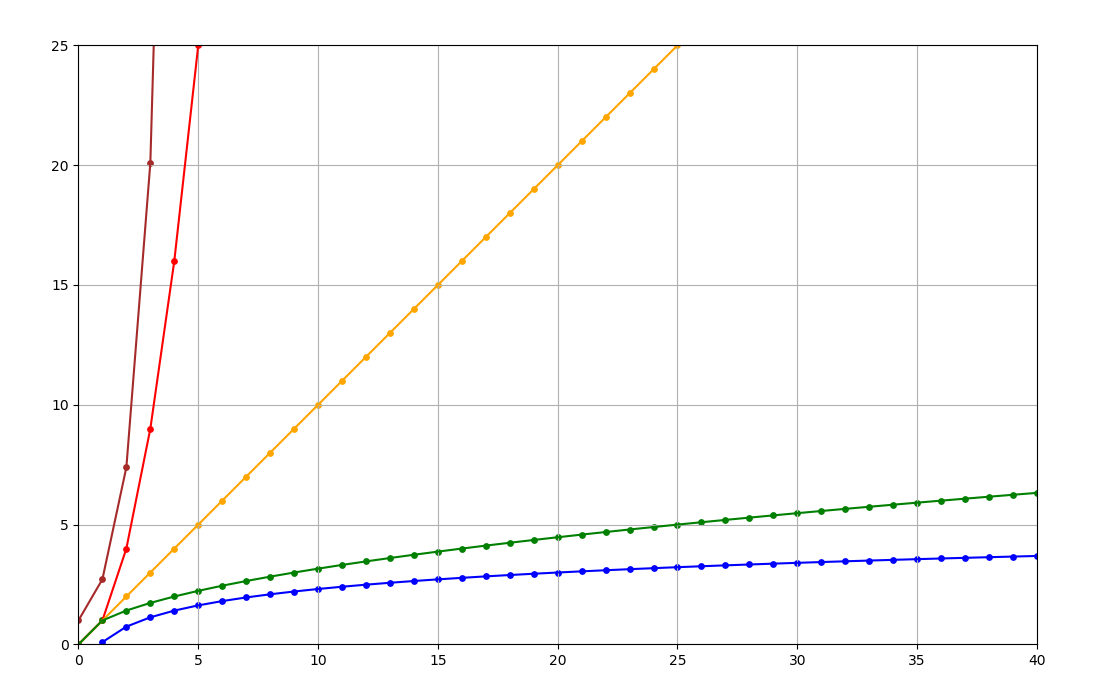
\includegraphics[scale=\myscale,scale=0.3]{figures/ecran-grandO}
 	
 	\emph{Les suites  $\ln(n)$, $\sqrt{n}$, $n$, $n^2$, $e^n$.}
 \end{center}
 
  
%--------------------------------------------------------------------
\subsection{Complexité d'un algorithme}

On mesure l'efficacité d'un algorithme à l'aide de la complexité. 

Nous définissons de manière informelle la complexité : la \defi{complexité}\index{complexite@complexité} d'un algorithme est le nombre d'opérations élémentaires exécutées.

\begin{itemize}
  \item Ce que l'on appelle \og{}opération élémentaire\fg{} peut varier selon le contexte : pour un calcul cela peut être le nombre de multiplications, pour un tri le nombre de comparaisons\ldots
	
	\item La complexité $C_n$ dépend de la taille $n$ des données en entrée (par exemple le nombre de chiffres d'un entier ou bien la longueur de la liste). On obtient ainsi une suite $(C_n)$.
	
	\item Les bons algorithmes ont des complexités polynomiales qui sont en $O(n)$ (linéaire), en $O(n^2)$ (quadratique) ou bien en $O(n^k)$, $k\in\Nn^*$ (polynomiale). Les mauvais algorithmes ont des complexités exponentielles, en $O(e^n)$ par exemple.
\end{itemize}


  
%--------------------------------------------------------------------
\subsection{Exemples de complexité}

\textbf{Multiplication de deux entiers.}

On souhaite multiplier deux entiers $a$ et $b$ de $n$ chiffres.
Il y a plusieurs méthodes, on les compare en comptant le nombre d'opérations élémentaires : ici les multiplications de petits nombres (entiers à $1$ ou $2$ chiffres).

\begin{center}
	\begin{tabular}{|c|c|}\hline
		Algorithme  & Ordre de la complexité \\ \hline\hline
		Multiplication d'école & $O(n^2)$ \\ \hline
		Multiplication de Karatsuba & $O(n^{\log_2(3)}) \simeq O(n^{1.58})$  \\ \hline
		Transformée de Fourier rapide & $O(n\cdot \ln(n) \cdot \ln(\ln(n)))$  \\\hline
	\end{tabular}
\end{center}  

Voici des exemples d'ordre de grandeur de la complexité pour différentes valeurs de $n$.
\begin{center}
	\begin{tabular}{|c|c|c|c|}\hline
		Algorithme  & $n=10$ & $n=100$ & $n=1000$  \\ \hline\hline
		Multiplication d'école & $100$ & $10\,000$ & $1\,000\,000$ \\ \hline
		Multiplication de Karatsuba & $38$ & $1478$ &  $56\,870$ \\ \hline
		Transformée de Fourier rapide & $19$ & $703$ & $13\,350$   \\\hline
	\end{tabular}
\end{center} 

Plus l'entier $n$ est grand, plus un bon algorithme prend l'avantage.

\bigskip

On termine par des exemples de problèmes et d'algorithmes correspondant à différentes classes de complexité.

\begin{center}
\begin{tabular}{|c|c|}
\hline
Complexité & Problème et algorithme \\ \hline\hline
\multirow{2}{*}{$O(1)$} & accès à un élément d'une liste de taille $n$ \\ 
                        & test si un nombre est pair ou impair \\ \hline
$O(\log_2(n))$          & recherche par dichotomie dans une liste ordonnée de taille $n$ \\ \hline
\multirow{2}{*}{$O(n)$} & recherche d'un maximum dans une liste non ordonnée  de taille $n$\\ 
                        & recherche si un élément  est présent dans une liste  de taille $n$\\ \hline
$O(n\log_2(n))$         & tri d'une liste  de taille $n$ par \emph{mergesort} \\ \hline   
\multirow{2}{*}{$O(n^2)$} & tri d'une liste  de taille $n$ par \emph{bubble sort}, \emph{selection sort}, \emph{insertion sort} \\ 
                        & recherche si un élément est présent en double dans une liste  de taille $n$\\ \hline
\multirow{2}{*}{$O(2^n)$} & problème du voyageur de commerce avec $n$ villes\\ 
                        & trouver tous les sous-ensembles de $\{1,2,\ldots,n\}$ \\ \hline  
% $O(n!)$         & trouver toutes les permutations de $\{1,2,\ldots,n\}$ \\ \hline                       
\end{tabular}
\end{center}

%Les deux dernière catégorie d'algorithme dont la complexité est en $O(2^n)$ ou en $O(n!)$  sont des compléxités exponentielle. 
La dernière catégorie d'algorithmes dont la complexité est en $O(2^n)$ est de complexité exponentielle (car $2^n = e^{n\ln2}$). 
Ce qui signifie que pour des valeurs de $n$ moyennes ou grandes, ces algorithmes sont inutilisables car ils n'aboutiront pas dans un temps raisonnable.


\bigskip
\bigskip
 	
\emph{Note.} Certains passages de cette section sont extraits du chapitre \og{}Tri -- Complexité\fg{} du livre \og{}Python au lycée (tome 2)\fg{}.

\end{document}
